\section{Queueing theoretic model}

One of the main outcomes of this research is the creation of a queueing network
model that consists of two waiting zones and accepts two types of individuals.

\begin{figure}[h]
    \centering
    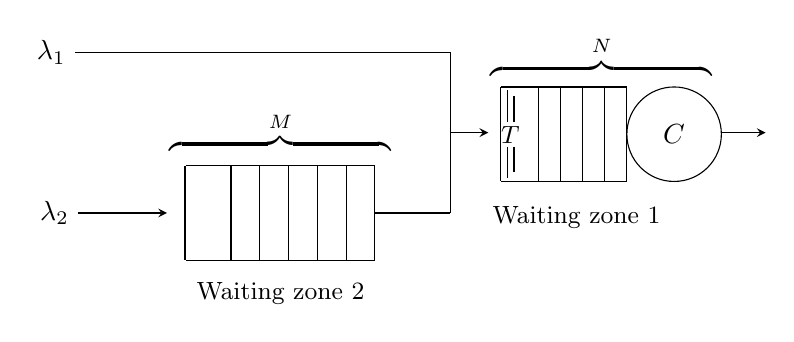
\begin{tikzpicture}[>=stealth, scale=0.8],
        % the rectangle of Queue 1
        \draw (0,0) -- ++(3cm,0) -- ++(0,-1.5cm) -- ++(-3cm,0);
        % The label above Queue 1 -> M
        \node[anchor=north] at (1.5cm, 1cm) {\(
            \overbrace{\qquad \qquad \qquad \qquad}^{M}
        \)};
        % The label below Queue 1 -> Waiting zone 2
        \node[anchor=north] at (1.5cm, -1.7cm) {\small{Waiting zone 2}};

        % the vertical lines in Queue 1
        \foreach \i in {1,...,5, 6.6}
        \draw (3cm-\i*13pt,0) -- +(0,-1.5cm);

        % % the circle in Queue 1
        % \draw (2.75,-0.75cm) circle [radius=0.75cm] node {\(0\)};

        % the rectangle in Queue 2
        \draw (5,1.25) -- ++(2cm,0) -- ++(0,-1.5cm) -- ++(-2cm,0);
        % the vertical lines in Queue 2
        \foreach \i in {1,...,4, 5.7}
        \draw (7cm-\i*10pt,1.25) -- +(0,-1.5cm);
        % The two vertical lines at the start of Queue 2
        \draw (7cm-54pt,1.2) -- +(0,-0.5cm);
        \draw (7cm-54pt,0.3) -- +(0,-0.5cm);
        \draw (7cm-51pt,1.1) -- +(0,-0.4cm);
        \draw (7cm-51pt,0.3) -- +(0,-0.4cm);

        % The label between the lines for T
        \node[anchor=north] at (5.15, 0.77 cm) {\small{\( T \)}};

        % The label above Queue 2 -> N
        \node[anchor=north] at (6.6cm, 2.2cm) {\(
            \overbrace{\qquad \qquad \qquad \qquad}^{N}
        \)};
        % The label below Queue 2 -> Waiting zone 1
        \node[anchor=north] at (6.2cm, -0.5cm) {\small{Waiting zone 1}};

        % the circle in Queue 2
        \draw (7.75,0.5) circle [radius=0.75cm] node {\(C\)};

        % Arrow line from Queue 2 outside
        \draw[->] (8.5,0.525) -- +(20pt,0);

        % Line from lambda_2 to Queue 1
        \draw[<-] (-0.3,-0.75) -- +(-40pt,0) node[left] {\( \lambda_2 \)};
        % First line (horizontal) after Queue 1
        \draw[-] (3,-0.75) -- +(34pt,0);
        % Second line (vertical) after Queue 1
        \draw (4.2, 0.525) -- (4.2, -0.75);

        % First line (horizontal) from lambda_1
        \draw (4.2, 1.8) -- +(-169.5pt,0) node[left] {\( \lambda_1 \)};
        % Second line (vertical) from lambda_1
        \draw (4.2, 1.8) -- (4.2, 0.525);
        % Arrow line to Queue 2
        \draw[->] (4.2, 0.525) -- (4.8, 0.525);
    \end{tikzpicture}
    \caption{A diagrammatic representation of the queueing model.
    The threshold \(T\) only applies to type 2 individuals.
    If the number of individuals in the hospital is \(T\), only
    individuals of type 1 are accepted (at a rate \(\lambda_1\)) and
    individuals of type 2 (arriving at a rate \(\lambda_2\)) are blocked in the
    parking space.}
    \label{fig:diagram_of_queueing_system}
\end{figure}


The model consists of two types of individuals; type 1 and type 2.
Type 1 individuals arrive instantly at waiting zone 1 and wait to receive their
service.
Type 2 individuals arrive at waiting zone 2 and wait there until they are
allowed to move to waiting zone 1.
They are allowed to proceed only when the number of
individuals in waiting zone 1 \textbf{and} in service is less than a
pre-determined threshold \(T\).
When the number of individuals is equal to or exceeds this threshold, all
type 2 individuals that arrive will stay \textit{blocked} in waiting zone 2
until the number of people in waiting zone 1 falls below \(T\).
This is shown diagrammatically in Figure \ref{fig:diagram_of_queueing_system}.
The parameters of the described queueing model are:

\begin{itemize}
    \item \(\lambda_i\): The arrival rate of type \(i\) individuals where
    \(i\in\{1, 2\}\)
    \item \(\mu\): The service rate for individuals receiving service at
    waiting zone 1
    \item \(C\): The number of servers
    \item \(T\): The threshold at which individuals of the second type are
    blocked
\end{itemize}

In chapter ?
% TODO: reference chapter \ref{ch:ed-ems-application}
this queueing network will be used to model the emergent behaviour between
Emergency Departments (EDs) and the Emergency Medical Systems (EMS).

\subsection{Discrete Event Simulation}
% TODO: Write DES subsection - emphasise on custom Node + include some code for
% node class

\subsection{Markov chain model}

A Markov chain is a stochastic model that is the primary analytical tool to 
study queues.
Under the assumption that all rates (arrival and service) are Markovian the
queueing system can be represented by a Markov chain
model~\cite{kemeny1976markov}.
The states of the Markov chain are denoted by \((u,v)\) where:

\begin{itemize}
    \item \(u\) is the number of individuals blocked in waiting zone 2
    \item \(v\) is the number of individuals either in waiting zone 1 or in the
    service centre
\end{itemize}

The set of all possible combination of pairs \((u, v)\) form all the possible 
states that the system can visit.
The state space of the Markov chain is denoted as the set \(S=S(T)\) which can
be written as the disjoint union:

\begin{align}
    S(T) =& S_1(T) \cup S_2(T) \text{ where:} \nonumber \\
    S_1(T) =& \left\{(0, v)\in\mathbb{N}_0^2 \; | \; v < T \right\}
    \label{eq:definition_of_S_as_disjoint_union} \\
    S_2(T) =& \{(u, v)\in\mathbb{N}_0^2 \; | \; v \geq T \} \nonumber
\end{align}

\(S_1\) consists of the set of states where the number of individuals in waiting
zone 1 is less than \(T\) (i.e. \(v < 0\)) and subsequently the number of
individuals in waiting zone 2 is zero (i.e. \(u = 0\)).
Similarly, \(S_2\) consists of the set of states where the number of individuals
in waiting zone 1 is greater than or equal to \(T\) (i.e. \(v \geq T\)) and 
hence it is possible for individuals to be at waiting zone 2 (i.e. 
\(u \geq 0\)).
This is illustrated diagrammatically in figure \ref{fig:general_markov_model}.

Having defined the set of states of the Markov chain model, the generator
matrix can also be obtained.
The generator matrix \(Q\) of the Markov chain consists of the
rates between the numerous states of the model.
Every entry \( Q_{ij} = Q_{(u_i, v_i),(u_j, v_j)} \) represents the rate from
state \( i = (u_i, v_i) \) to state \( j = (u_j , v_j) \) for all
\( (u_i, v_i), (u_j, v_j) \in S \).
The entries of \(Q\) can be calculated using the state-mapping function
described in equation (\ref{eq:markov_transition_rate}).
Here \(\Lambda\) denotes the overall arrival rate in the model for
both types of individuals (i.e. \(\Lambda = \lambda_1 + \lambda_2\)).

\begin{equation} \label{eq:markov_transition_rate}
    Q_{ij} =
    \begin{cases}
        \Lambda, & \textbf{if } (u_i, v_i) - (u_j, v_j) = (0,-1) \textbf{ and }
        v_i < \text{t} \\
        \lambda_1, & \textbf{if } (u_i, v_i) - (u_j, v_j) = (0,-1)
        \textbf{ and } v_i \geq \text{t} \\
        \lambda_2, & \textbf{if } (u_i, v_i) - (u_j, v_j) = (-1,0) \\
        v_i \mu, & \textbf{if } (u_i, v_i) - (u_j, v_j) = (0,1) \textbf{ and }
        v_i \leq C \textbf{ or} \\ & \hspace{0.37cm}(u_i, v_i) - (u_j, v_j) =
        (1,0) \textbf{ and } v_i = T \leq C \\
        C \mu, & \textbf{if } (u_i, v_i) - (u_j, v_j) = (0,1) \textbf{ and }
        v_i > C
        \textbf{ or} \\ & \hspace{0.37cm}(u_i, v_i) - (u_j, v_j) = (1,0)
        \textbf{ and } v_i = T > C\\
        -\sum_{j=1}^{|Q|}{Q_{ij}} & \textbf{if } i = j \\
        0, & \textbf{otherwise}
    \end{cases}
\end{equation}

Note that for large values of \(N\) and \(M\) most of the entries of the
transition matrix will be zero.
In order to speed up the computation of the transition matrix, instead of
considering every possible pair of states in the state space a new function
that maps a state to every possible destination state can be used.
Equation (\ref{eq:state_map_to_destination_states}) maps a state \((u, v)\)
to all possible destination states that the system can go to when on that state.

\begin{equation}\label{eq:state_map_to_destination_states}
    \mathcal{M}(u, v) = 
    \begin{cases}
        \{(u, v + 1), (u, v - 1)\} & \textbf{if } v < T \\
        \{(u + 1, v), (u, v + 1), (u, v - 1)\} & \textbf{if } v = T 
        \textbf{ and } u = 0 \\
        \{(u + 1, v), (u, v + 1), (u - 1, v)\} & \textbf{if } v = T
        \textbf{ and } u > 0 \\
        \{(u, v + 1), (u + 1, v), (u, v - 1)\} & \textbf{if } v > T \\
    \end{cases}
\end{equation}


A visualisation of how the transition rates relate to the states of the model
can be seen in the general Markov chain model shown in Figure
\ref{fig:general_markov_model}.

\begin{figure}[H]
    \centering
    \scalebox{.8}
    {
        \begin{tikzpicture}[-, node distance = 0.9cm, auto, every node/.style={scale=0.7}]

            % Markov chain variables
            \tikzmath{
                let \initdist = 0.5cm;
                let \altdist = 1.2cm;
                let \minsz = 1.6cm;
            }

            % S_1 and S_2 rectangles
            \tikzmath{
                let \leftOne = -0.8;
                let \rightOne = 2.7;
                let \upOne = 0.8;
                let \downOne = -2.7;
                let \leftTwo = 2.8;
                let \rightTwo = 13;
                let \upTwo = -2.95;
                let \downTwo = -16.4;
            }

            % General case variables
            \tikzmath{
                let \GCsmallx = 8.3;
                let \GCsmally = -9.5;
                let \GCbigx = 4.1;
                let \GCbigy = -11.8;
            }

            % Rectangle for S1
            \draw[ultra thin, dashed] (\leftOne, \downOne) -- (\leftOne, \upOne);
            \draw[ultra thin, dashed] (\leftOne, \upOne) -- (\rightOne, \upOne);
            \draw[ultra thin, dashed] (\rightOne, \upOne) -- node 
            {\Huge{\( \quad S_1 \)}}(\rightOne, \downOne);
            \draw[ultra thin, dashed] (\rightOne, \downOne) -- (\leftOne, \downOne);

            % Rectangle for S2
            \draw[ultra thin, dashed] (\leftTwo, \downTwo) -- node 
            {\Huge{\( S_2 \quad \)}}(\leftTwo, \upTwo);
            \draw[ultra thin, dashed] (\leftTwo, \upTwo) -- (\rightTwo, \upTwo);
            \draw[ultra thin, dashed] (\rightTwo, \upTwo) -- (\rightTwo, \downTwo);
            \draw[ultra thin, dashed] (\rightTwo, \downTwo) -- (\leftTwo, \downTwo);

            % Small square of general case
            \draw [thick] (\GCsmallx, \GCsmally) -- node {} 
            (\GCsmallx + 0.4, \GCsmally);
            \draw [thick] (\GCsmallx + 0.4, \GCsmally) -- node {} 
            (\GCsmallx + 0.4, \GCsmally - 0.4);
            \draw [thick] (\GCsmallx + 0.4, \GCsmally - 0.4) -- node {} 
            (\GCsmallx, \GCsmally - 0.4);
            \draw [thick] (\GCsmallx, \GCsmally - 0.4) -- node {} 
            (\GCsmallx, \GCsmally);


            % Dashed lines to from small square to big one 
            \draw [ultra thin] (\GCsmallx, \GCsmally) -- node {} 
            (\GCbigx, \GCbigy);
            \draw [ultra thin] (\GCsmallx + 0.4, \GCsmally) -- node {} 
            (\GCbigx + 4, \GCbigy);
            \draw [ultra thin] (\GCsmallx, \GCsmally - 0.4) -- node {} (7, \GCbigy);
            \draw [ultra thin] (\GCsmallx + 0.4, \GCsmally - 0.4) -- node {} 
            (\GCbigx + 4, \GCbigy - 4);
            
            % Big Square of general case
            \draw [ultra thick] (\GCbigx, \GCbigy) -- node {} (\GCbigx + 4, \GCbigy);
            \draw [ultra thick] (\GCbigx + 4, \GCbigy) -- node {} 
            (\GCbigx + 4, \GCbigy - 4);
            \draw [ultra thick] (\GCbigx + 4, \GCbigy - 4) -- node {General Case} 
            (\GCbigx, \GCbigy - 4);
            \draw [ultra thick] (\GCbigx, \GCbigy - 4) -- node {} (\GCbigx, \GCbigy);

            % First Line
            \node[state, minimum size=1.5cm] (zero) {(0,0)};
            \node[state, node distance = \initdist, minimum size=\minsz, below right=of zero] 
            (one) {(0,1)};
            \node[draw=none, node distance = \initdist, minimum size=\minsz, below right=of one] 
            (two) {\textbf{\( \ddots \)}};
            \node[state, node distance = \initdist, minimum size=\minsz, below right=of two] 
            (three) {(0,T)};
            \node[state, node distance = \altdist, minimum size=\minsz, right=of three] 
            (four) {(0,T+1)};
            \node[draw=none, node distance = \altdist, minimum size=\minsz, right=of four] 
            (five) {\textbf{\dots}};
            \node[state, minimum size=\minsz, right=of five] (six) {(0,C)};
            \node[draw=none, minimum size=\minsz, right=of six] (seven) {\textbf{\dots}};

            % Second Line
            \node[state, minimum size=\minsz, below=of three] (three_one) {(1,T)};
            \node[state, minimum size=\minsz, below=of four] (four_one) {(1,T+1)};
            \node[draw=none, minimum size=\minsz, below=of five] (five_one) {\textbf{\dots}};
            \node[state, minimum size=\minsz, right=of five_one] (six_one) {(1,C)};
            \node[draw=none, minimum size=\minsz, right=of six_one] (seven_one) {\textbf{\dots}};
            
            % Third Line
            \node[state, minimum size=\minsz, below=of three_one] (three_two) {(2,T)};
            \node[state, minimum size=\minsz, below=of four_one] (four_two) {(2,T+1)};
            \node[draw=none, minimum size=\minsz, below=of five_one] (five_two) 
            {\textbf{\dots}};
            \node[state, minimum size=\minsz, right=of five_two] (six_two) {(2,C)};
            \node[draw=none, minimum size=\minsz, right=of six_two] (seven_two) 
            {\textbf{\dots}};

            % Fourth line
            \node[draw=none, node distance = \altdist, minimum size=\minsz, below=of three_two] 
            (three_three) {\textbf{\vdots}};
            \node[draw=none, node distance = \altdist, minimum size=\minsz, below=of four_two] 
            (four_three) {\textbf{\vdots}};
            \node[draw=none, node distance = 2cm, minimum size=\minsz, below=of five_two] 
            (five_three) {};
            \node[draw=none, node distance = \altdist, minimum size=\minsz, below=of six_two] 
            (six_three) {\textbf{\vdots}};

            % Fifth line
            \node[draw=none, node distance = 0.3cm, minimum size=\minsz, below=of four_three] 
            (general_case_up) {};
            \node[state, node distance = \altdist, minimum size=\minsz, below=of general_case_up] 
            (general_case_mid) {\( (u_i, v_i) \)};

            \node[draw=none, node distance = \altdist, minimum size=\minsz, below=of general_case_mid] 
            (general_case_down) {};
            \node[draw=none, node distance = \altdist, minimum size=\minsz, left=of general_case_mid] 
            (general_case_left) {};
            \node[draw=none, node distance = \altdist, minimum size=\minsz, right=of general_case_mid] 
            (general_case_right) {};

            \draw[every loop]
                % First Horizontal Edges
                (zero) edge[bend left] node {\( \Lambda \)} (one)
                (one) edge[bend left] node {\( \mu \)} (zero)
                (one) edge[bend left] node {\( \Lambda \)} (two)
                (two) edge[bend left] node {\( 2 \mu \)} (one)
                (two) edge[bend left] node {\( \Lambda \)} (three)
                (three) edge[bend left] node {\( T \mu \)} (two)
                (three) edge[bend left] node {\( \lambda_1 \)} (four)
                (four) edge[bend left] node {\( (T+1) \mu \)} (three)
                (four) edge[bend left] node {\( \lambda_1 \)} (five)
                (five) edge[bend left] node {\( (T+2) \mu \)} (four)
                (five) edge[bend left] node {\( \lambda_1 \)} (six)
                (six) edge[bend left] node {\( C\mu \)} (five)
                (six) edge[bend left] node {\( \lambda_1 \)} (seven)
                (seven) edge[bend left] node {\( C\mu \)} (six)

                % Second Horizontal Edges
                (three_one) edge[bend left] node {\( \lambda_1 \)} (four_one)
                (four_one) edge[bend left] node {\( (T+1) \mu \)} (three_one)
                (four_one) edge[bend left] node {\( \lambda_1 \)} (five_one)
                (five_one) edge[bend left] node {\( (T+2) \mu \)} (four_one)
                (five_one) edge[bend left] node {\( \lambda_1 \)} (six_one)
                (six_one) edge[bend left] node {\( C\mu \)} (five_one)
                (six_one) edge[bend left] node {\( \lambda_1 \)} (seven_one)
                (seven_one) edge[bend left] node {\( C\mu \)} (six_one)

                % Third Horizontal Edges
                (three_two) edge[bend left] node {\( \lambda_1 \)} (four_two)
                (four_two) edge[bend left] node [below] {\( (T+1) \mu \)} (three_two)
                (four_two) edge[bend left] node {\( \lambda_1 \)} (five_two)
                (five_two) edge[bend left] node {\( (T+2) \mu \)} (four_two)
                (five_two) edge[bend left] node {\( \lambda_1 \)} (six_two)
                (six_two) edge[bend left] node {\( C\mu \)} (five_two)
                (six_two) edge[bend left] node {\( \lambda_1 \)} (seven_two)
                (seven_two) edge[bend left] node {\( C\mu \)} (six_two)

                % First Vertical Edges
                (three) edge[bend left] node {\( \lambda_2 \)} (three_one)
                (three_one) edge[bend left] node {\( T \mu \)} (three)
                (three_one) edge[bend left] node {\( \lambda_2 \)} (three_two)
                (three_two) edge[bend left] node {\( T\mu \)} (three_one)
                (three_two) edge[bend left] node {\( \lambda_2 \)} (three_three)
                (three_three) edge[bend left] node {\( T\mu \)} (three_two)

                % Second Vertical Edges
                (four) edge node {\( \lambda_2 \)} (four_one)
                (four_one) edge node {\( \lambda_2 \)} (four_two)
                (four_two) edge node {\( \lambda_2 \)} (four_three)

                % Fourth Vertical Edges
                (six) edge node {\( \lambda_2 \)} (six_one)
                (six_one) edge node {\( \lambda_2 \)} (six_two)
                (six_two) edge node {\( \lambda_2 \)} (six_three)

                % General Case
                (general_case_left) edge[bend left] node {\( \lambda_1 \)} (general_case_mid)
                (general_case_mid) edge[bend left] node {\( v_i \mu \)} (general_case_left)
                (general_case_right) edge[bend left] node {\( (v_i +1) \mu \)} (general_case_mid)
                (general_case_mid) edge[bend left] node {\( \lambda_1 \)} (general_case_right)
                % (five_three) edge node {\( \lambda_2 \)} (general_case_mid)
                (general_case_up) edge node {\( \lambda_2 \)} (general_case_mid)
                (general_case_mid) edge node {\( \lambda_2 \)} (general_case_down)
                ;
        \end{tikzpicture}
    }
    \caption{General case of the Markov chain model} 
    \label{fig:general_markov_model}
\end{figure}


In order to consider this model numerically an adjustment needs to be made.
The problem defined above assumes no upper boundary to the number of individuals
that can wait for service or for the ones that are blocked in waiting zone 2.
Therefore, a different state space \( \tilde S \) is constructed where
\( \tilde S \subseteq S \) and there is a maximum allowed number of individuals
\(N\) that can be in waiting zone 1 and a maximum allowed number of individuals
\(M\) that can be blocked in waiting zone 2:

\begin{equation}\label{eq:truncated_state_space}
    \tilde S = \left\{ (u, v) \in S\;| u \leq M, v\leq N \right\}
\end{equation}

The adjusted Markov chain model with states \(\tilde S\) can be seen in Figure
\ref{fig:adjusted_markov_model}.

\begin{figure}[H]
    \centering
    \scalebox{.8}
    {
        \begin{tikzpicture}[-, node distance = 0.9cm, auto, every node/.style={scale=0.7}]

            % Markov chain variables
            \tikzmath{
                let \initdist = 0.9cm;
                let \altdist = 0.9cm;
                let \minsz = 1.8cm;
            }


            % First Line
            \node[state, minimum size=\minsz] (one) {(0,0)};
            \node[draw=none, node distance = \initdist, minimum size=\minsz, right=of one] 
            (two) {\textbf{\dots}};
            \node[state, node distance = \initdist, minimum size=\minsz, right=of two] 
            (three) {(0,T)};
            \node[draw=none, node distance = \altdist, minimum size=\minsz, right=of three] 
            (four) {\textbf{\dots}};
            \node[state, node distance = \altdist, minimum size=\minsz, right=of four] 
            (five) {(0, C)};
            \node[draw=none, minimum size=\minsz, right=of five] (six) {\textbf{\dots}};
            \node[state, minimum size=\minsz, right=of six] (seven) {(0, N)};

            % Second Line
            \node[state, minimum size=\minsz, below=of three] (three_one) {(1,T)};
            \node[draw=none, minimum size=\minsz, below=of four] (four_one) {\textbf{\dots}};
            \node[state, minimum size=\minsz, below=of five] (five_one) {(1, C)};
            \node[draw=none, minimum size=\minsz, right=of five_one] (six_one) {\textbf{\dots}};
            \node[state, minimum size=\minsz, right=of six_one] (seven_one) {(1, N)};
            
            % Third Line
            \node[draw=none, minimum size=\minsz, below=of three_one] (three_two) {\textbf{\vdots}};
            \node[draw=none, minimum size=\minsz, below=of four_one] (four_two) {\textbf{\(\ddots\)}};
            \node[draw=none, minimum size=\minsz, below=of five_one] (five_two) 
            {\textbf{\vdots}};
            \node[draw=none, minimum size=\minsz, right=of five_two] (six_two) {\textbf{\(\ddots\)}};
            \node[draw=none, minimum size=\minsz, right=of six_two] (seven_two) 
            {\textbf{\vdots}};

            % Fourth line
            \node[state, node distance = \altdist, minimum size=\minsz, below=of three_two] 
            (three_three) {(M, T)};
            \node[draw=none, node distance = \altdist, minimum size=\minsz, below=of four_two] 
            (four_three) {\textbf{\dots}};
            \node[state, node distance = \altdist, minimum size=\minsz, below=of five_two] 
            (five_three) {(M, C)};
            \node[draw=none, node distance = \altdist, minimum size=\minsz, below=of six_two] 
            (six_three) {\textbf{\dots}};
            \node[state, node distance = \altdist, minimum size=\minsz, below=of seven_two] 
            (seven_three) {(M, N)};

            \draw[every loop]
                % First Horizontal Edges
                (one) edge[bend left] node {\( \Lambda \)} (two)
                (two) edge[bend left] node {\( 2 \mu \)} (one)
                (two) edge[bend left] node {\( \Lambda \)} (three)
                (three) edge[bend left] node {\( T \mu \)} (two)
                (three) edge[bend left] node {\( \lambda_1 \)} (four)
                (four) edge[bend left] node {\( (T+1) \mu \)} (three)
                (four) edge[bend left] node {\( \lambda_1 \)} (five)
                (five) edge[bend left] node {\( C\mu \)} (four)
                (five) edge[bend left] node {\( \lambda_1 \)} (six)
                (six) edge[bend left] node {\( C\mu \)} (five)
                (six) edge[bend left] node {\( \lambda_1 \)} (seven)
                (seven) edge[bend left] node {\( C\mu \)} (six)

                % Second Horizontal Edges
                (three_one) edge[bend left] node {\( \lambda_1 \)} (four_one)
                (four_one) edge[bend left] node {\( (T+1) \mu \)} (three_one)
                (four_one) edge[bend left] node {\( \lambda_1 \)} (five_one)
                (five_one) edge[bend left] node {\( C\mu \)} (four_one)
                (five_one) edge[bend left] node {\( \lambda_1 \)} (six_one)
                (six_one) edge[bend left] node {\( C\mu \)} (five_one)
                (six_one) edge[bend left] node {\( \lambda_1 \)} (seven_one)
                (seven_one) edge[bend left] node {\( C\mu \)} (six_one)

                % Third Horizontal Edges
                (three_three) edge[bend left] node {\( \lambda_1 \)} (four_three)
                (four_three) edge[bend left] node [below] {\( (T+1) \mu \)} (three_three)
                (four_three) edge[bend left] node {\( \lambda_1 \)} (five_three)
                (five_three) edge[bend left] node {\( C\mu \)} (four_three)
                (five_three) edge[bend left] node {\( \lambda_1 \)} (six_three)
                (six_three) edge[bend left] node {\( C\mu \)} (five_three)
                (six_three) edge[bend left] node {\( \lambda_1 \)} (seven_three)
                (seven_three) edge[bend left] node {\( C\mu \)} (six_three)

                % First Vertical Edges
                (three) edge[bend left] node {\( \lambda_2 \)} (three_one)
                (three_one) edge[bend left] node {\( T \mu \)} (three)
                (three_one) edge[bend left] node {\( \lambda_2 \)} (three_two)
                (three_two) edge[bend left] node {\( T\mu \)} (three_one)
                (three_two) edge[bend left] node {\( \lambda_2 \)} (three_three)
                (three_three) edge[bend left] node {\( T\mu \)} (three_two)

                % Second Vertical Edges
                (five) edge node {\( \lambda_2 \)} (five_one)
                (five_one) edge node {\( \lambda_2 \)} (five_two)
                (five_two) edge node {\( \lambda_2 \)} (five_three)

                % Fourth Vertical Edges
                (seven) edge node {\( \lambda_2 \)} (seven_one)
                (seven_one) edge node {\( \lambda_2 \)} (seven_two)
                (seven_two) edge node {\( \lambda_2 \)} (seven_three)
                ;
        \end{tikzpicture}
    }
    \caption{Adjusted case of the Markov chain model} 
    \label{fig:adjusted_markov_model}
\end{figure}



\subsubsection{Steady state probability vector \(\pi\)}

The generator matrix \( Q \) defined in (\ref{eq:markov_transition_rate}) can
be used to get the probability vector \( \pi \) that contains the steady state
probabilities of the Markov chain model.
The vector \( \pi \) is commonly used to study stochastic systems and it's main
purpose is to keep track of the probability of being at any given state of
the Markov chain model.
\(\pi_i\) is the steady state probability of being in state \((u_i, v_i) \in
\tilde S\) which is the \(i^{\text{th}}\) state of \(\tilde S\) for some
ordering of \(\tilde S\).
The term \textbf{steady state} refers to the instance of the vector \( \pi \)
where the probabilities of being at any state becomes stable over time.
Thus, by considering the steady state vector \( \pi \) the relationship between
it and \( Q \) is given by:

\begin{equation}\label{eq:steady_state_from_generator_matrix}
    \frac{d\pi}{dt} = \pi Q = \vec{0}
\end{equation}


\subsubsection{Numerical integration approach}

Another method that can be used to get the steady state probability vector is
to solve the differential equation from equation
\ref{eq:steady_state_from_generator_matrix} numerically.
Two methods of solving the differential equation were considered.
Both methods observe the value of \(\pi\) over time until it
reaches the steady state based on some initial starting value \(\pi_0\):

\begin{gather}
    \frac{d\pi}{dt} = \pi Q \\
    \pi(t_0) = \pi_0 \nonumber \\
    \text{where } \pi_0 = 
    [\frac{1}{|\pi|}, \frac{1}{|\pi|}, \dots, \frac{1}{|\pi|}] \nonumber
\end{gather}

Two types of methods were considered to solve the differential equation
numerically.
The first method uses a combination of Adams' method~\cite{adams_method} and the
backward differentiation formula (BDF)~\cite{backward_differentiation_formula}.
This method is generally used to solve systems of the form
\(\frac{dy}{dt} = f\) with a dense or banded Jacobian when the problem is stiff,
which then uses the BDF algorithm, while when the problem is non-stiff it uses
Adams' method.
This was implemented using \textit{scipy.integrate. odeint} from the python
library \textit{SciPy}~\cite{2020SciPy-NMeth} that uses the
\textit{lsoda}~\cite{lsoda_algorithm} integration method.

The second approach uses the explicit Runge-Kutta integration method of order 5
by controlling the error assuming accuracy of order 4
\cite{solve_ivp_rk45_method, runge_kutta_formulas}.
The general recursive formula for the explicit family of Runge-Kutta methods is
given by:

\begin{equation}
    y_{n+1} = y_n + h \sum_{i=1}^s b_i k_i
\end{equation}
\begin{align}
    k_1 & = f(t_n, y_n), \nonumber \\
    k_2 & = f(t_n+c_2h, y_n+h(a_{21}k_1)), \nonumber \\
    k_3 & = f(t_n+c_3h, y_n+h(a_{31}k_1+a_{32}k_2)), \nonumber \\
        & \ \ \vdots \nonumber \\
    k_s & = f(t_n+c_s h, y_n+h(a_{s1}k_1+a_{s2}k_2+\cdots+a_{s,s-1}k_{s-1})) 
    \nonumber
\end{align}

where \(y_0\) is the given initial value, \(s\) is the number of stages and
\(h\) is the step size.
The coefficients \(b_i\), \(c_i\), and \(a_{ij}\) are usually arranged in a
mnemonic device known as the Butcher's tableau.
This was implemented using \textit{scipy.integrate. solve\_ivp} from the python
library \textit{SciPy}~\cite{2020SciPy-NMeth}.


\subsubsection{Linear algebraic approach}

The steady state probability vector \( \pi \) can be obtained by solving the
linear equation:

\begin{equation}\label{eq:numpy_linalg_solve_1}
    Q^T \pi = \vec{0} \hspace{0.5cm} \text{such that} \hspace{0.5cm} 
    \sum_{i} \pi_i = 1
\end{equation}

The two equations can be combined into one by augmenting the matrix \( Q^T \)
in such a way that it includes the extra constraint \( \sum_i \pi_i = 1 \).
The new augmented matrix \(\tilde Q\) is defined as \(Q\) with the final
column replaced with a vector of ones and vector \(\vec{b}\) is defined
as a column vector of \(0\)s apart from the final element which is \(1\).
Note that, \(\tilde Q\) needs to be a square matrix in order to solve the
equation using linear algebra (i.e. the matrix needs to be invertible).
Thus, the steady state probability vector can be calculated by solving the
linear equation:

\begin{equation}
    \tilde Q^T \pi = \vec{b}
\end{equation}

Using LU decomposition with partial pivoting and row interchanges, matrix
\(Q^T\) can be expressed of the form \(P \times L \times U\), where \(P\) is
a permutation matrix, \(L\) is a unit lower triangular matrix, and \(U\) is
an upper triangular matrix~\cite{strang2006linear}.
The factored form of \(Q^T\) can then be used to solve the system.
This was implemented using \textit{numpy.linalg.solve} from the
python library \textit{numpy} \cite{2020NumPy-Array} \cite{lapack99}.


\subsubsection{Least squares approach}

Another approach that is considered is the least squares method. 
As the problem becomes more complex (i.e. as the artificial parameters \(N\)
and \(M\) defined in equation \ref{eq:truncated_state_space} increase)
the computational time required to solve it increases by a lot.
Thus, one may obtain a good approximation of the steady state vector \( \pi \)
by solving the following equation:

\begin{equation}
    \pi = \text{argmin}_{\pi \in \mathbb{R}^{|\pi|}}\|\tilde Q^T \pi - b\|_2^2
\end{equation}

The above expression gets the vector \( \pi \) that approximately solves 
equation \(\tilde Q^T \pi = b\).
This was implemented using \textit{numpy.linalg.lstsq} from the python 
library \textit{numpy}~\cite{2020NumPy-Array}.

\subsubsection{Closed-form approach}
% TODO: Write closed form section to get steady state

\subsection{Performance measures}
Using vector \(\pi\) there are numerous performance measures of the model that
can be calculated.
The following equations utilise \(\pi\) to get performance measures on the
average number of individuals in waiting zone 1 and in waiting zone 2:

\begin{itemize}
    \item Mean number of individuals in the entire system:
        \begin{equation}
            L_S = \sum_{i=1}^{|\pi|} \pi_i (u_i + v_i)
        \end{equation}
    \item Mean number of individuals in waiting zone 1:
        \begin{equation}
            L_1 = \sum_{i=1}^{|\pi|} \pi_i v_i
        \end{equation}
    \item Mean number of individuals in waiting zone 2:
        \begin{equation}
            L_2 = \sum_{i=1}^{|\pi|} \pi_i u_i
        \end{equation}
\end{itemize}

Consequently, there are some additional performance measures of interest that
are not as straightforward to calculate.
Such performance measures are the mean waiting time in the system (for both
type 1 and type 2 individuals), the mean time blocked in waiting zone 2 (only
valid for type 2 individuals) and the proportion of individuals that wait in
waiting zone 1 within a predefined time target (for both types).

\subsubsection{Waiting time}
% TODO: Write waiting time subsection

\subsubsection{Blocking time}
% TODO: Write blocking time subsection

\subsubsection{Proportion of individuals within target}
% TODO: Write proportion of individuals within target subsection


\subsection{Numeric results and timings}
% TODO: Write numeric results and timings section (compare DES with Markov)


\subsection{ED-EMS application}
% TODO: Write ED-EMS application subsection